\documentclass{ULBreport} % Llama a tu plantilla adaptada

% Configuración de enlaces (esto sí se queda en el main o se puede mover al .cls)
\hypersetup{
    colorlinks=true,
    linkcolor=black,
    filecolor=magenta,      
    urlcolor=blue,
    citecolor=black,
}

\begin{document}

% 1. GENERAR LA PORTADA CON EL COMANDO ESTRUCTURADO
\titleUCLM{
    title={Valorant Role Compliance Evaluation (VRCE):\\ Un sistema de Inteligencia Artificial para la estimación probabilística del cumplimiento del rol en esports},
    course={Desarrollo e Integración de Servicios de IA},
    author={{\large Nicolás Celis Moreno}\\[0.7em]
            {\large Erick Mesias Rosero Lesano}\\[0.7em]
            {\large Johann Ismael Ordoñez Echeverría}\\[0.7em]},
    teacher={Julio Alberto López},
    date={2026},
    logoL={Logo_UCLM_40.jpg},
    logoR={esi.png},
    watermark={uclm_fondo.png}
}

% 2. ÍNDICES (Se generan con cuadro gris automáticamente al usar la clase report)
\tableofcontents
\listoftables
\listoffigures


% -----------------------------------------------------------------
% 3. CONTENIDO PRINCIPAL
% -----------------------------------------------------------------
\chapter{Definición del problema y determinación del alcance}

En este capítulo se presenta la definición del problema abordado en el proyecto \textit{VRCE -- Valorant Role Compliance Evaluation}, así como la determinación de su alcance, viabilidad y estudio del retorno sobre la inversión. El objetivo es establecer una base conceptual, operativa y económica sólida para el desarrollo de un sistema de inteligencia artificial orientado a estimar la probabilidad de cumplimiento del rol de un jugador en competiciones de \textit{Valorant}.

\section{Definición del proyecto}

\subsection{Contexto del problema}

En el entorno competitivo de los \textit{esports}, y en particular en el videojuego \textit{Valorant}, los equipos de nivel Tier 2 operan bajo condiciones de alta exigencia táctica, donde cada jugador cumple una función específica dentro de la estructura del equipo. En este contexto, la correcta ejecución del rol asignado ---\textit{Duelist}, \textit{Controller}, \textit{Sentinel} o \textit{Initiator}--- resulta determinante para el desempeño colectivo.

Sin embargo, la evaluación habitual de los jugadores suele apoyarse en métricas generales como el KDA, el ACS o el daño promedio por ronda. Aunque estas métricas aportan información útil, no permiten determinar de forma directa si un jugador está cumpliendo las responsabilidades propias de su rol. Por ejemplo, un \textit{Duelist} y un \textit{Sentinel} no deben ser evaluados bajo los mismos criterios, ya que sus responsabilidades tácticas dentro de la partida son distintas.

Esta situación genera un problema relevante para los equipos Tier 2: la evaluación del jugador puede quedar condicionada por métricas aisladas, comparaciones inadecuadas entre roles o valoraciones subjetivas del \textit{staff} técnico. Como consecuencia, decisiones relacionadas con alineaciones, entrenamientos, scouting o ajustes tácticos pueden tomarse sin una medición suficientemente objetiva del cumplimiento funcional del jugador.

En consecuencia, el problema central del proyecto no consiste en medir el rendimiento general del jugador, sino en estimar de forma objetiva y contextualizada la probabilidad de cumplimiento del rol. Para ello, el sistema VRCE utiliza métricas de rendimiento, variables derivadas y modelos de aprendizaje automático que permiten transformar datos históricos de partidas en una medida interpretable de cumplimiento del rol.

% FIGURA 1.1
\begin{figure}[H]
    \centering
    
\includegraphics[width=0.9\textwidth]{figura1.png}
    \caption{Arquitectura general del sistema VRCE: flujo desde el dataset, entrenamiento del modelo, API de inferencia y generación de resultados.}
    \label{fig:arquitectura}
\end{figure}

\subsection{Cliente y usuarios}

El cliente principal del sistema son los equipos de \textit{esports} de nivel Tier 2, específicamente su \textit{staff} técnico, compuesto por analistas y entrenadores. Estos usuarios son quienes utilizarán la información generada por el sistema para apoyar decisiones relacionadas con el análisis táctico, la revisión del desempeño funcional de los jugadores y la planificación de entrenamientos.

Adicionalmente, los propios jugadores pueden actuar como usuarios secundarios del sistema, ya que los resultados pueden ayudarles a comprender mejor su grado de adaptación al rol que desempeñan. No obstante, el enfoque principal del sistema está orientado al cuerpo técnico, debido a que este grupo es responsable de interpretar los resultados y convertirlos en decisiones operativas dentro del equipo.

Los usuarios del sistema poseen conocimientos técnicos sobre las métricas del juego; sin embargo, requieren una presentación clara, estructurada y accionable de la información para reducir la dependencia de interpretaciones subjetivas.

\subsection{Decisión que soporta el sistema}

El sistema desarrollado proporcionará al \textit{staff} técnico una estimación objetiva del cumplimiento del rol de cada jugador. Esta información permite apoyar decisiones relacionadas con la evaluación funcional del jugador dentro de la estructura táctica del equipo.

Entre las decisiones que el sistema está diseñado para apoyar, se destacan las siguientes:

\begin{enumerate}
    \item Determinar si un jugador está cumpliendo adecuadamente las responsabilidades asociadas a su rol.
    \item Identificar desviaciones en el cumplimiento del rol a partir de métricas de rendimiento y variables contextuales.
    \item Comparar jugadores dentro de un mismo rol, evitando comparaciones incorrectas entre funciones distintas.
    \item Apoyar decisiones de alineación, rotación, entrenamiento y seguimiento individual.
    \item Complementar procesos de scouting mediante una medida funcional basada en datos.
\end{enumerate}

% FIGURA 1.2
\begin{figure}[H]
    \centering
    
\includegraphics[width=0.8\textwidth]{figura2.png}
    \caption{Objetivos del sistema VRCE para la estimación objetiva del cumplimiento del rol en \textit{Valorant}.}
    \label{fig:objetivos}
\end{figure}

El sistema no sustituye el criterio del analista o entrenador, sino que actúa como una herramienta de apoyo para fundamentar decisiones mediante evidencia cuantitativa.

\subsection{Descripción del sistema propuesto}

El sistema propuesto, denominado \textit{VRCE -- Valorant Role Compliance Evaluation}, consiste en una solución de inteligencia artificial orientada a estimar la probabilidad de cumplimiento del rol de un jugador de \textit{Valorant}. Para ello, el sistema procesa datos históricos de partidas, realiza limpieza y transformación de variables, calcula una etiqueta de cumplimiento del rol mediante reglas heurísticas y entrena modelos de aprendizaje automático supervisado.

A nivel técnico, el sistema se estructura en dos componentes principales. El primero corresponde al módulo de entrenamiento, encargado de procesar el dataset, generar las variables necesarias, calcular el \textit{role score}, normalizar la variable objetivo y entrenar el modelo. El segundo corresponde al módulo de inferencia, implementado mediante una API REST en NodeJS, que recibe los datos de un jugador y devuelve la probabilidad estimada de cumplimiento del rol.

El sistema se despliega mediante contenedores Docker separados para entrenamiento e inferencia, lo que permite mantener una arquitectura modular y reproducible. Además, la API se encuentra documentada mediante Swagger/OpenAPI, facilitando su prueba, comprensión e integración con otros sistemas.

Como resultado de su ejecución, el sistema genera las siguientes salidas:

\begin{enumerate}
    \item \textbf{Probabilidad de cumplimiento del rol:} valor continuo normalizado en el intervalo $[0,1]$ que representa el grado en que el jugador satisface las responsabilidades asociadas a su rol.
    \item \textbf{Reporte analítico:} información estructurada sobre el comportamiento del jugador en relación con las métricas utilizadas por el modelo.
    \item \textbf{Respuesta mediante API REST:} salida consumible por otros sistemas o interfaces mediante un endpoint de inferencia.
\end{enumerate}

\subsection{Definición de éxito y fracaso}

El sistema se considerará exitoso si cumple con los siguientes criterios:

\begin{enumerate}
    \item Estimar de forma consistente la probabilidad de cumplimiento del rol.
    \item Presentar resultados coherentes con el conocimiento experto del dominio.
    \item Permitir la interpretación de las variables que más influyen en la estimación del modelo.
    \item Reducir la dependencia de evaluaciones puramente subjetivas.
    \item Proporcionar una API funcional, documentada y desplegable mediante contenedores.
\end{enumerate}

Por el contrario, el sistema se considerará un fracaso si genera estimaciones inconsistentes, si no diferencia adecuadamente los comportamientos esperados por rol, si no aporta valor frente al análisis manual tradicional, si presenta resultados difíciles de interpretar o si la arquitectura de inferencia no resulta funcional para su uso operativo.

\section{Determinación del alcance}

\subsection{Datos del sistema}

El sistema opera sobre datos reales de partidas de \textit{Valorant}, obtenidos a partir de fuentes especializadas como Riot API, HenrikDev API, VLR.gg y Tracker.gg. El dataset contiene métricas individuales de rendimiento, entre ellas ACS, ADR, KPR, APR, FKPR, FDPR, porcentaje de disparos a la cabeza, éxito en situaciones de clutch, asesinatos, muertes, asistencias y agentes utilizados.

El dataset original no contiene directamente una variable de rol ni una etiqueta explícita de cumplimiento. Por ello, el sistema realiza un proceso de limpieza y transformación que incluye corrección de tipos de datos, extracción de variables derivadas, cálculo de KDR, procesamiento de clutches, mapeo de agentes a roles y generación de una variable objetivo normalizada.

\subsection{Alcance funcional}

El sistema desarrollado en el marco del presente proyecto incluye las siguientes funcionalidades:

\begin{itemize}
    \item Limpieza y preprocesamiento del dataset original.
    \item Mapeo de agentes a roles de \textit{Valorant}.
    \item Cálculo de un \textit{role score} mediante reglas heurísticas.
    \item Normalización del score al rango $[0,1]$.
    \item Entrenamiento de modelos de aprendizaje automático para estimar la probabilidad de cumplimiento del rol.
    \item Serialización del modelo entrenado para su uso posterior.
    \item Implementación de una API REST para inferencia.
    \item Separación del sistema en contenedores de entrenamiento e inferencia mediante Docker.
    \item Documentación de la API mediante Swagger/OpenAPI.
\end{itemize}

\subsection{Limitaciones del sistema}

Con el propósito de mantener un alcance realista y controlado, el sistema no incluye predicción de resultados de partidas, simulación de escenarios de juego, recomendación automática de agentes o roles, ni toma de decisiones autónoma.

Asimismo, el sistema se basa en métricas estadísticas disponibles en el dataset, por lo que no incorpora análisis directo de video, comunicación del equipo, posicionamiento espacial detallado, uso específico de habilidades ni lectura táctica completa de cada ronda. Estas limitaciones no invalidan el sistema, pero delimitan el tipo de conclusiones que pueden derivarse de sus resultados.

\subsection{Justificación del alcance}

El alcance definido permite abordar el problema central de forma concreta y viable: estimar la probabilidad de cumplimiento del rol de un jugador a partir de métricas disponibles y procesables. La separación entre entrenamiento e inferencia permite construir una arquitectura modular, reproducible y más cercana a un entorno de despliegue real.

Además, el uso de Docker facilita la ejecución del sistema en distintos entornos, mientras que la API REST documentada con Swagger permite que el modelo pueda ser consumido por otros sistemas o interfaces. De este modo, el proyecto no se limita a un análisis en notebook, sino que propone una solución funcional con capacidad de integración.

\section{Viabilidad y estudio del ROI}

\subsection{Viabilidad del proyecto}

\subsubsection{Viabilidad técnica}

El proyecto presenta viabilidad técnica debido a que utiliza herramientas ampliamente disponibles y adecuadas para el problema planteado. El procesamiento de datos y el entrenamiento del modelo se realizan en Python, utilizando librerías especializadas para análisis de datos y aprendizaje automático. La inferencia se expone mediante una API REST desarrollada en NodeJS, lo que facilita su integración con aplicaciones externas.

El uso de Docker permite separar el entorno de entrenamiento del entorno de inferencia, reduciendo problemas de dependencias y favoreciendo la reproducibilidad del sistema. Además, la documentación con Swagger/OpenAPI facilita la prueba de los endpoints y mejora la mantenibilidad de la solución.

La arquitectura técnica del sistema se compone de los siguientes elementos:

\begin{itemize}
    \item Python para limpieza, transformación, entrenamiento y serialización del modelo.
    \item Modelos de aprendizaje automático para estimar la probabilidad de cumplimiento del rol.
    \item NodeJS y Express para la construcción de la API REST.
    \item Docker para separar los contenedores de entrenamiento e inferencia.
    \item Swagger/OpenAPI para documentar y probar la API.
\end{itemize}

En consecuencia, no se identifican barreras técnicas significativas para la ejecución del proyecto en un entorno académico o experimental.

\subsubsection{Viabilidad operativa}

Desde el punto de vista operativo, el sistema se integra de forma natural en los flujos de trabajo de equipos Tier 2. Los analistas y entrenadores ya trabajan con métricas de rendimiento, por lo que VRCE no introduce una lógica completamente ajena, sino que reorganiza dichas métricas alrededor del cumplimiento del rol.

Además, al ofrecer una API de inferencia, el sistema puede integrarse posteriormente con interfaces web, dashboards o herramientas internas de análisis. Esto permite que el sistema funcione como una herramienta de apoyo, sin reemplazar el criterio experto del \textit{staff} técnico.

\subsubsection{Viabilidad económica}

Los equipos de nivel Tier 2 suelen operar con recursos limitados, por lo que una herramienta de análisis debe ser proporcional, accesible y justificable. El sistema propuesto presenta un costo reducido debido al uso de tecnologías abiertas, infraestructura ligera y contenedores reproducibles.

El costo de operación puede mantenerse bajo, ya que el modelo no requiere infraestructura de alto rendimiento para realizar inferencias. Una vez entrenado, el sistema puede ejecutarse como una API ligera, lo que reduce los costos asociados a despliegue y mantenimiento.

\subsection{Estimación de costos}

Considerando que el equipo está compuesto por tres desarrolladores y que la duración estimada de la fase inicial del proyecto es de entre cuatro y seis semanas, los costos hipotéticos de desarrollo se situarían entre 3.000 y 9.000 dólares en concepto de recursos humanos, con una inversión adicional de entre 50 y 200 dólares en infraestructura inicial. Esto resulta en un costo total estimado de entre 3.050 y 9.200 dólares.

En cuanto a los costos operativos recurrentes, se estima un gasto mensual de entre 10 y 50 dólares para \textit{hosting}, backend e infraestructura básica, con costos mínimos de mantenimiento durante la fase inicial del despliegue.

\begin{table}[H]
    \centering
    \caption{Estimación de costos iniciales del proyecto}
    \label{tab:costos}
    \begin{tabular}{|l|l|}
        \hline
        \textbf{Concepto} & \textbf{Estimación} \\ \hline
        Desarrollo (3 personas) & \$3,000 -- \$9,000 USD \\ \hline
        Infraestructura inicial & \$50 -- \$200 USD \\ \hline
        Total estimado & \$3,050 -- \$9,200 USD \\ \hline
    \end{tabular}
\end{table}

\subsection{Estudio del ROI (Return on Investment)}

\subsubsection{Beneficios esperados}

El sistema aporta valor en tres dimensiones principales. La primera corresponde a la reducción de subjetividad en la evaluación del jugador, ya que introduce una medida cuantitativa centrada en el cumplimiento del rol. La segunda se relaciona con la optimización del tiempo de análisis, debido a que automatiza parte del procesamiento y permite obtener una estimación rápida mediante una API. La tercera corresponde a la mejora en la toma de decisiones, especialmente en procesos de entrenamiento, seguimiento de jugadores y scouting funcional.

Para equipos Tier 2, donde los recursos de análisis suelen ser más limitados que en organizaciones de primer nivel, una herramienta de este tipo puede aportar valor al reducir tareas repetitivas y mejorar la consistencia de las evaluaciones.

\subsubsection{Estimación del ROI}

Si bien el retorno sobre la inversión es difícil de cuantificar con precisión en términos económicos directos, puede estimarse de forma cualitativa a partir del ahorro de tiempo y de la mejora en la calidad de las decisiones. Si el sistema contribuye a evitar una decisión errónea de alineación, entrenamiento o fichaje, el ahorro generado puede superar el costo operativo de la herramienta.

Además, al estar construido con tecnologías de bajo costo y una arquitectura ligera, el sistema presenta una relación favorable entre inversión y utilidad potencial. Su capacidad de despliegue mediante Docker y su exposición mediante API REST permiten escalar su uso sin requerir una infraestructura costosa, lo que refuerza su viabilidad económica para equipos Tier 2.

% -----------------------------------------------------------------
% HITO 2: MODELADO DEL PROBLEMA Y ANÁLISIS DEL DATASET
% -----------------------------------------------------------------
\chapter{Modelado del problema y análisis del dataset}

En este capítulo se desarrolla la formulación técnica del problema, la comprensión inicial del conjunto de datos, el análisis exploratorio, la detección de sesgos, las limitaciones del dataset y las decisiones de preparación necesarias para el posterior modelado del sistema \textit{VRCE -- Valorant Role Compliance Evaluation}. Esta fase constituye un paso previo indispensable antes del entrenamiento de modelos, ya que permite justificar la calidad, pertinencia y restricciones de los datos utilizados.

\section{Formulación del problema}

El problema se modela como una tarea de regresión supervisada cuyo objetivo es estimar la probabilidad de cumplimiento del rol de un jugador en una partida específica. Esta probabilidad se representa como un valor continuo en el intervalo $[0,1]$, donde valores cercanos a 1 indican un mayor grado de cumplimiento de las responsabilidades asociadas al rol.

Formalmente, el problema puede expresarse como:

\[
P(\text{cumplimiento del rol} \mid X)
\]

donde $X$ representa el conjunto de características observables del jugador en una partida determinada, incluyendo métricas ofensivas, métricas de soporte, métricas de riesgo, variables críticas y variables categóricas como el agente y el rol.

A partir de esta estimación, el sistema puede comparar jugadores dentro de un mismo rol, evitando comparaciones incorrectas entre funciones tácticas diferentes, como \textit{Duelist}, \textit{Controller}, \textit{Sentinel} e \textit{Initiator}.

\section{Justificación del dataset seleccionado}

El dataset seleccionado corresponde a estadísticas reales de jugadores de \textit{Valorant}, obtenidas a partir de fuentes especializadas de seguimiento competitivo. Este conjunto de datos resulta adecuado para el problema planteado porque contiene métricas individuales directamente relacionadas con el comportamiento del jugador durante las partidas, tales como daño promedio por ronda, asesinatos por ronda, asistencias, primeras bajas, primeras muertes, porcentaje de disparos a la cabeza y desempeño en situaciones de clutch.

El dataset original contiene 17.996 registros y 25 columnas, donde cada fila representa el rendimiento agregado de un jugador en un contexto competitivo determinado. Entre las variables originales se incluyen:

\begin{itemize}
    \item \textit{Tournament}, \textit{Stage}, \textit{Match Type}, \textit{Player}, \textit{Teams} y \textit{Agents}.
    \item \textit{Rounds Played}, \textit{Rating}, \textit{Average Combat Score} y \textit{Average Damage Per Round}.
    \item \textit{Kills Per Round}, \textit{Assists Per Round}, \textit{First Kills Per Round} y \textit{First Deaths Per Round}.
    \item \textit{Headshot \%}, \textit{Clutch Success \%}, \textit{Clutches (won/played)}, \textit{Kills}, \textit{Deaths}, \textit{Assists}, \textit{First Kills} y \textit{First Deaths}.
\end{itemize}

La selección de este dataset se justifica porque permite construir una aproximación funcional al cumplimiento del rol a partir de métricas observables. Sin embargo, el dataset no contiene una etiqueta explícita de cumplimiento del rol, por lo que es necesario aplicar una estrategia de supervisión débil basada en reglas heurísticas y conocimiento del dominio.

\section{Análisis exploratorio de datos}

El análisis exploratorio se realiza con el objetivo de comprender la naturaleza de los datos antes de aplicar cualquier modelo de aprendizaje automático. En esta fase se inspecciona la estructura del dataset, se analizan sus tipos de datos, se identifican valores nulos, duplicados y se calculan medidas estadísticas descriptivas.

Inicialmente, se revisan las dimensiones del dataset, los nombres de las columnas y la información general de tipos de datos mediante funciones de inspección como \texttt{info()} y \texttt{describe()}. Este análisis permite identificar que algunas variables se encuentran en formatos que requieren transformación, como porcentajes almacenados como texto o la columna \textit{Clutches (won/played)}, que contiene dos valores en una misma cadena.

\subsection{Medidas estadísticas descriptivas}

Se calculan medidas estadísticas sobre las variables numéricas relevantes, incluyendo media, desviación estándar, valores mínimos, máximos y percentiles. Este análisis permite observar la dispersión de métricas como \textit{Average Combat Score}, \textit{Average Damage Per Round}, \textit{Kills Per Round}, \textit{Assists Per Round}, \textit{First Kills Per Round}, \textit{First Deaths Per Round}, \textit{Headshot \%}, \textit{Clutch Success \%}, \textit{Clutch\_Success\_Ratio}, \textit{Clutches\_Won} y \textit{KDR}.

La revisión estadística evidencia que las variables presentan escalas distintas y comportamientos heterogéneos. Por ejemplo, algunas métricas ofensivas presentan mayor dispersión, mientras que métricas como asistencias o primeras muertes tienen rangos más acotados. Esta diferencia de escalas justifica la posterior normalización de variables y el uso de modelos capaces de manejar relaciones no lineales.

\subsection{Distribución de roles y agentes}

Dado que el dataset original no contiene una variable explícita de rol, se realiza un mapeo de agentes a roles. A partir de esta transformación se obtiene la variable \textit{Role}, la cual clasifica a los jugadores según el agente utilizado en una de las cuatro categorías principales del juego: \textit{Duelist}, \textit{Controller}, \textit{Sentinel} e \textit{Initiator}.

% FIGURA 2.1
\begin{figure}[H]
    \centering
    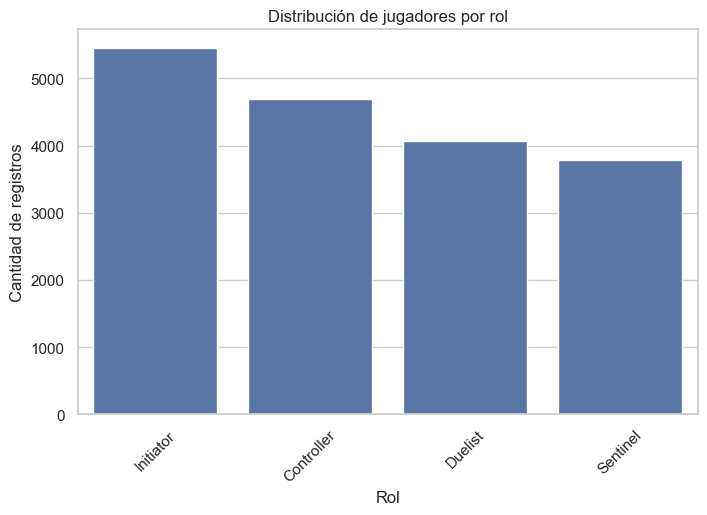
\includegraphics[width=0.8\textwidth]{data_charts/output1.png}
    \caption{Jugadores por rol}
    \label{fig:objetivos}
\end{figure}

Posteriormente, se analiza la distribución de registros por rol y la frecuencia de aparición de agentes. Este análisis es importante porque permite detectar posibles desequilibrios en la representación de los roles. Una distribución desbalanceada puede afectar el aprendizaje del modelo, ya que los roles con mayor cantidad de registros pueden tener mayor influencia durante el entrenamiento.

% FIGURA 2.2
\begin{figure}[H]
    \centering
    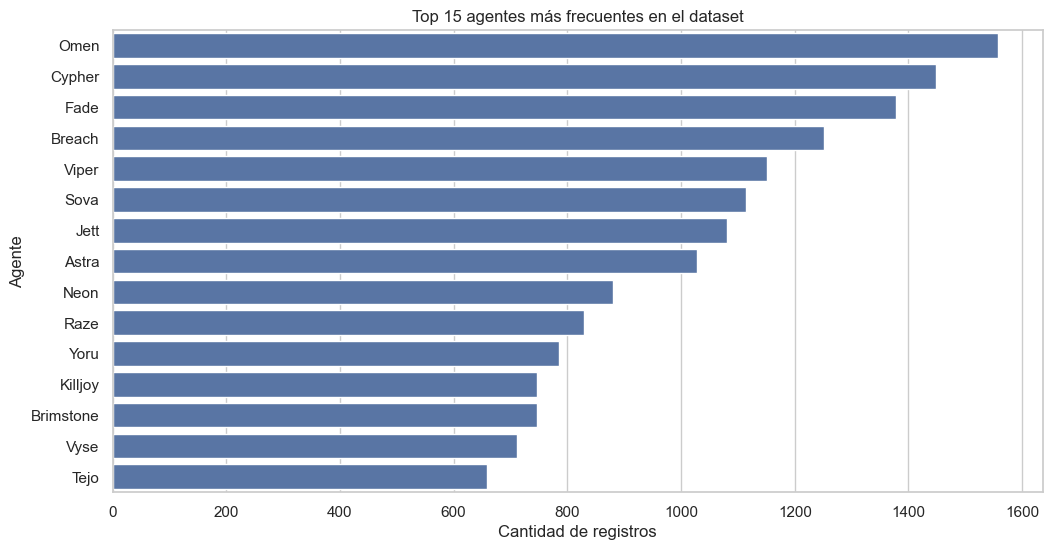
\includegraphics[width=0.8\textwidth]{data_charts/output2.png}
    \caption{Top agentes mas frecuentes}
    \label{fig:objetivos}
\end{figure}

\subsection{Distribución de variables clave}

Se generan histogramas para analizar variables relevantes como \textit{Average Combat Score}, \textit{Average Damage Per Round}, \textit{Kills Per Round}, \textit{Assists Per Round}, \textit{First Kills Per Round}, \textit{First Deaths Per Round} y \textit{KDR}. Estas visualizaciones permiten observar que las variables no siguen necesariamente una distribución normal, lo cual es esperable en datos competitivos de videojuegos, donde el rendimiento puede variar según rol, agente, mapa, rival y contexto de partida.

La presencia de distribuciones asimétricas y comportamientos no lineales refuerza la necesidad de utilizar modelos capaces de capturar relaciones complejas entre variables.

% FIGURA 2.3
\begin{figure}[H]
    \centering
    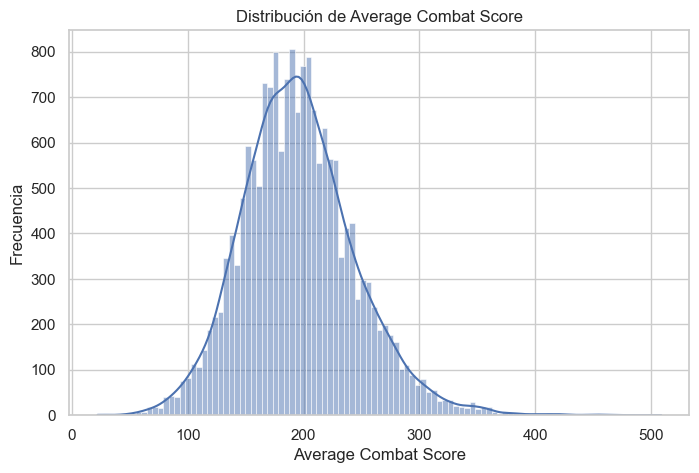
\includegraphics[width=0.8\textwidth]{data_charts/output3.png}
    \caption{Promedio de combate}
    \label{fig:objetivos}
\end{figure}

% FIGURA 2.4
\begin{figure}[H]
    \centering
    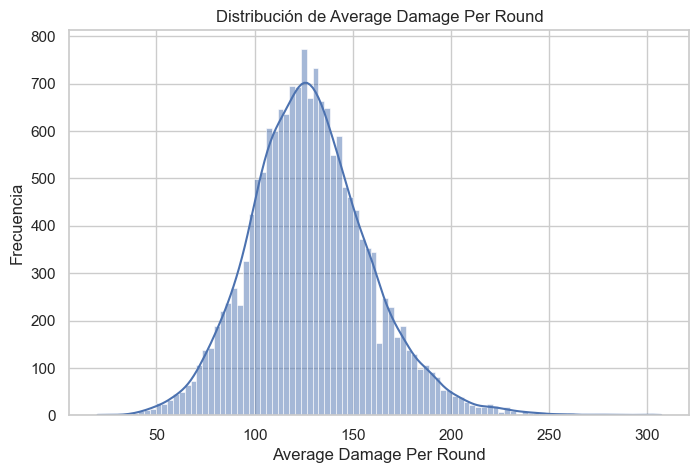
\includegraphics[width=0.8\textwidth]{data_charts/output4.png}
    \caption{Promedio de daño por ronda}
    \label{fig:objetivos}
\end{figure}

% FIGURA 2.5
\begin{figure}[H]
    \centering
    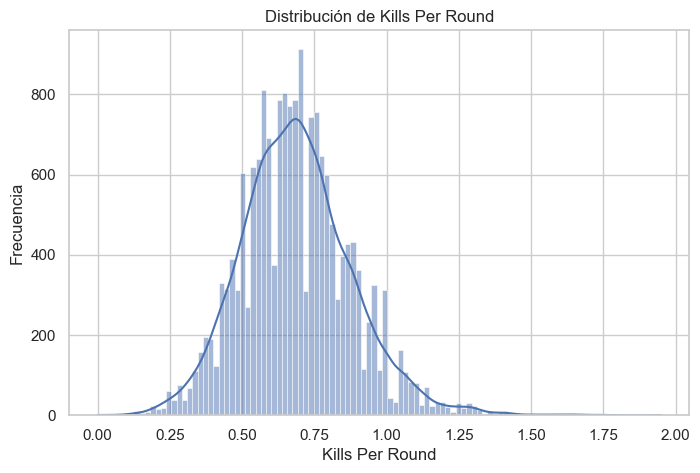
\includegraphics[width=0.8\textwidth]{data_charts/output5.png}
    \caption{Muerte por ronda}
    \label{fig:objetivos}
\end{figure}

% FIGURA 2.6
\begin{figure}[H]
    \centering
    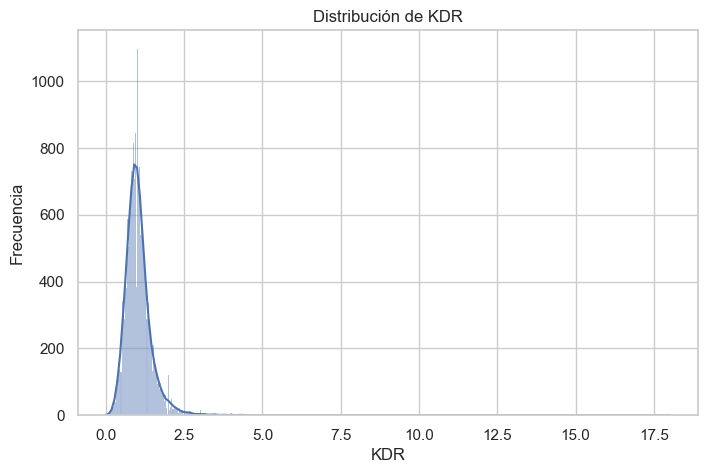
\includegraphics[width=0.8\textwidth]{data_charts/output6.png}
    \caption{KDR}
    \label{fig:objetivos}
\end{figure}

\subsection{Análisis de outliers}

Se utilizan diagramas de caja para detectar valores atípicos en variables como \textit{Average Combat Score}, \textit{Average Damage Per Round}, \textit{Kills Per Round}, \textit{First Kills Per Round}, \textit{First Deaths Per Round} y \textit{KDR}. Los outliers identificados no se eliminan automáticamente, ya que pueden representar partidas reales con desempeños excepcionalmente altos o bajos.

Esta decisión es relevante en el dominio de los \textit{esports}, donde un jugador puede tener actuaciones extremas debido a diferencias tácticas, nivel del rival, duración de la partida o rol desempeñado. Por ello, los valores atípicos se conservan, pero se tienen en cuenta al seleccionar modelos robustos frente a variabilidad.

\subsection{Correlación entre variables}

Se calcula una matriz de correlación entre las variables numéricas seleccionadas. Este análisis permite identificar relaciones entre métricas ofensivas, de soporte y de riesgo. Por ejemplo, es esperable encontrar relaciones entre \textit{Kills Per Round}, \textit{Average Damage Per Round} y \textit{Average Combat Score}, ya que todas reflejan componentes ofensivos del rendimiento.

La matriz de correlación también permite detectar posibles redundancias entre variables, lo cual es útil para la fase de selección de características. Sin embargo, no se descartan variables únicamente por correlación, ya que algunas pueden tener importancia diferente dependiendo del rol evaluado.

% FIGURA 2.7
\begin{figure}[H]
    \centering
    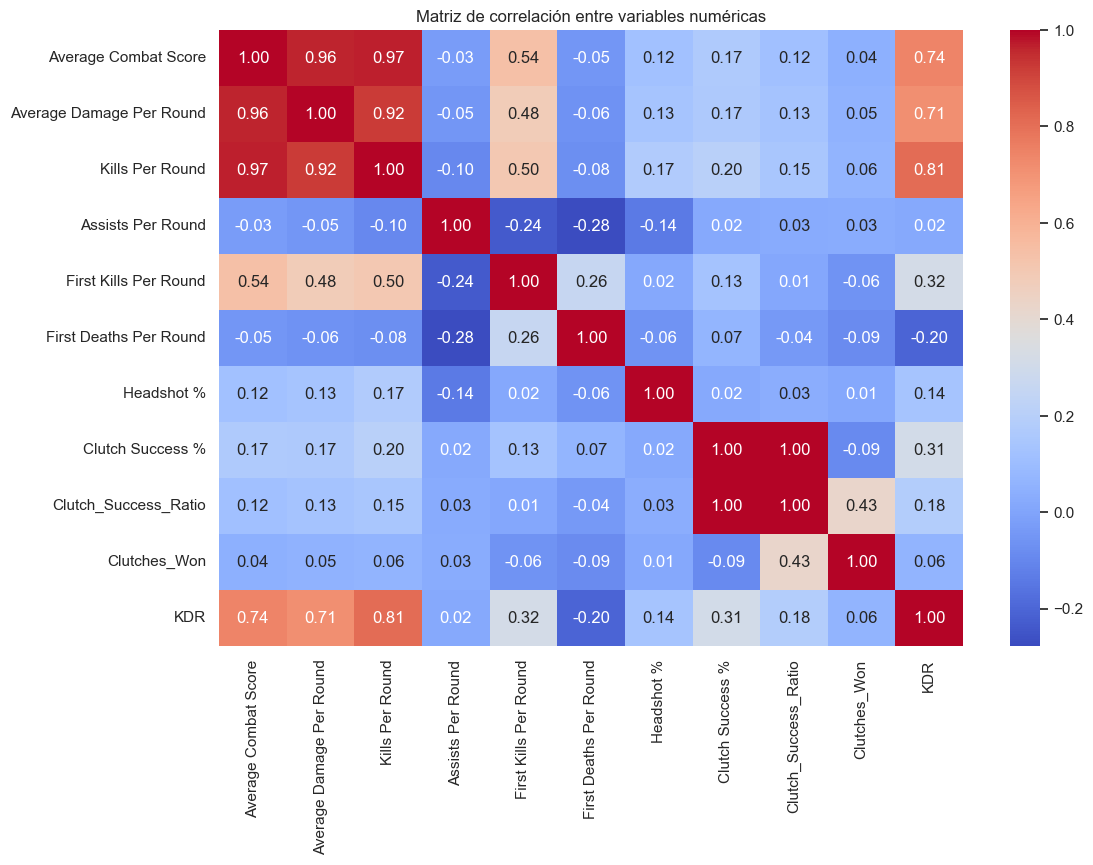
\includegraphics[width=0.8\textwidth]{data_charts/output7.png}
    \caption{Matriz de correlación}
    \label{fig:objetivos}
\end{figure}

\section{Detección de sesgos en los datos}

El análisis del dataset permite identificar varios posibles sesgos que deben considerarse antes del modelado:

\begin{itemize}
    \item \textbf{Sesgo por rol:} la cantidad de registros puede no estar equilibrada entre \textit{Duelist}, \textit{Controller}, \textit{Sentinel} e \textit{Initiator}. Esto puede provocar que el modelo aprenda con mayor precisión los patrones de los roles más representados.
    
    \item \textbf{Sesgo por agente:} algunos agentes aparecen con mayor frecuencia que otros, lo que puede afectar la representación de estilos de juego específicos dentro de cada rol.
    
    \item \textbf{Sesgo competitivo:} el dataset se enfoca en datos competitivos de \textit{Valorant}, por lo que sus conclusiones son más adecuadas para contextos similares y no necesariamente generalizables a jugadores casuales.
    
    \item \textbf{Sesgo temporal:} si los datos corresponden a distintos periodos competitivos, los cambios de meta, balance de agentes y estrategias pueden afectar la interpretación de las métricas.
    
    \item \textbf{Sesgo de etiquetado:} la variable \textit{Role} no existe originalmente en el dataset, sino que se genera mediante un mapeo de agentes a roles. Esta decisión introduce una aproximación basada en conocimiento del dominio.
\end{itemize}

Estos sesgos no invalidan el dataset, pero delimitan el alcance de las conclusiones y justifican la necesidad de interpretar los resultados del modelo con cautela.

\section{Limitaciones del dataset}

Aunque el dataset contiene métricas relevantes para aproximar el cumplimiento del rol, presenta limitaciones importantes para resolver completamente el problema planteado. Entre las principales limitaciones se encuentran:

\begin{itemize}
    \item No contiene datos espaciales de posicionamiento durante las rondas.
    \item No incluye análisis de video o revisión de VODs.
    \item No contiene información sobre comunicación del equipo.
    \item No incluye uso detallado de habilidades por ronda.
    \item No dispone de información económica avanzada.
    \item No posee una etiqueta real de cumplimiento del rol validada por expertos.
\end{itemize}

Estas limitaciones implican que el sistema no puede evaluar de forma completa todos los aspectos tácticos del jugador. En consecuencia, VRCE aproxima el cumplimiento del rol a partir de métricas estadísticas disponibles, utilizando supervisión débil para generar la variable objetivo.

\section{Limpieza y preprocesamiento}

El preprocesamiento del dataset incluye la corrección de tipos de datos, la transformación de porcentajes, el tratamiento de columnas compuestas y la creación de variables derivadas.

En primer lugar, las columnas porcentuales como \textit{Headshot \%}, \textit{Clutch Success \%} y \textit{Kill, Assist, Trade, Survive \%} se convierten a valores numéricos. Posteriormente, las columnas numéricas se transforman mediante conversión explícita, controlando errores de formato.

La columna \textit{Clutches (won/played)} se separa en dos variables derivadas: \textit{Clutches\_Won} y \textit{Clutches\_Played}. A partir de ellas se calcula \textit{Clutch\_Success\_Ratio}, que representa la proporción de clutches ganados respecto a los jugados.

También se calcula la variable \textit{KDR}, definida como la relación entre asesinatos y muertes. Esta variable resume la eficiencia general del jugador en enfrentamientos directos.

\section{Ingeniería de variables}

La ingeniería de variables se realiza con el objetivo de transformar el dataset original en una representación más adecuada para el problema de cumplimiento del rol. Además de conservar métricas originales relevantes, se generan variables derivadas que permiten representar dimensiones funcionales del jugador.

Entre las variables derivadas se incluyen:

\begin{itemize}
    \item \textbf{Clutch\_Success\_Ratio:} mide la proporción de situaciones de clutch ganadas.
    \item \textbf{Clutches\_Won:} representa el número de clutches ganados.
    \item \textbf{KDR:} resume la relación entre asesinatos y muertes.
    \item \textbf{Offensive\_Index:} aproxima el impacto ofensivo del jugador.
    \item \textbf{Support\_Index:} aproxima el aporte de soporte mediante asistencias y desempeño en situaciones críticas.
    \item \textbf{Risk\_Index:} aproxima el riesgo asumido por el jugador en función de primeras muertes y eficiencia de bajas.
    \item \textbf{Survival\_Index:} representa la capacidad de supervivencia relativa.
    \item \textbf{Clutch\_Index:} resume el impacto del jugador en situaciones críticas.
\end{itemize}

Estas variables permiten enriquecer la representación del jugador y conectar las estadísticas disponibles con comportamientos esperados dentro de cada rol.

\section{Selección de variables}

Las variables finales seleccionadas para el modelado son:

\begin{itemize}
    \item \textit{Average Combat Score}
    \item \textit{Average Damage Per Round}
    \item \textit{Kills Per Round}
    \item \textit{Assists Per Round}
    \item \textit{First Kills Per Round}
    \item \textit{First Deaths Per Round}
    \item \textit{Headshot \%}
    \item \textit{Clutch Success \%}
    \item \textit{Clutch\_Success\_Ratio}
    \item \textit{Clutches\_Won}
    \item \textit{KDR}
    \item \textit{Agents}
    \item \textit{Role}
\end{itemize}

Las variables \textit{Agents} y \textit{Role} se codifican mediante \textit{Label Encoding} para permitir su uso en modelos de aprendizaje automático. Esta selección combina métricas ofensivas, de soporte, de riesgo, de precisión, de impacto crítico y variables contextuales.

\subsection{Selección automática de características}

Además de la selección manual basada en conocimiento del dominio, se aplica un método automático de selección de características mediante \textit{SelectKBest} con la función estadística \textit{f\_regression}. Este método permite estimar la relación individual entre cada variable predictora y la variable objetivo \textit{role\_score}.

El uso de selección automática permite contrastar si las variables elegidas manualmente presentan relevancia estadística respecto al objetivo del modelo. Las variables con mayor puntuación se consideran más informativas para explicar la probabilidad de cumplimiento del rol.

Este análisis no reemplaza el criterio de dominio, pero aporta una validación adicional sobre la pertinencia de las variables seleccionadas.

% FIGURA 2.8
\begin{figure}[H]
    \centering
    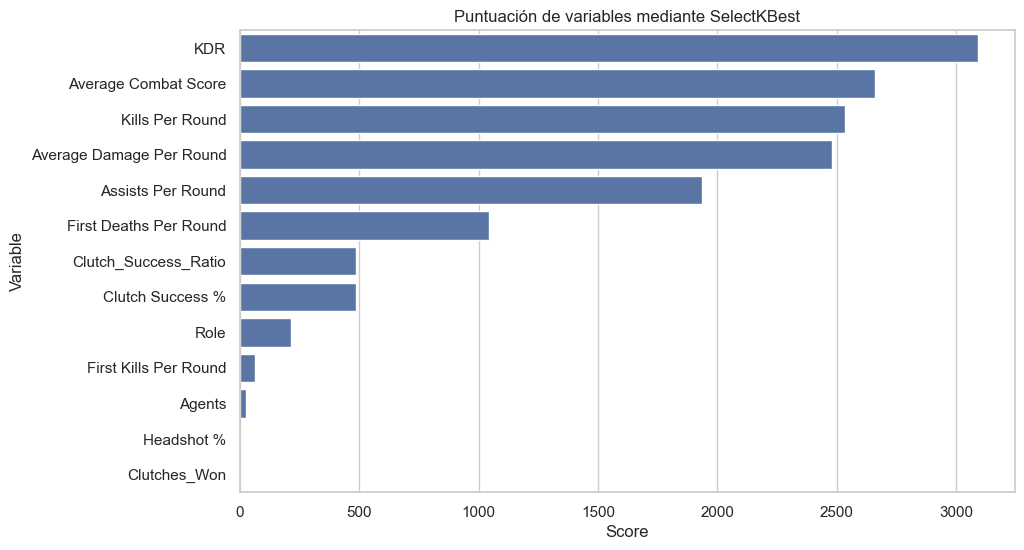
\includegraphics[width=0.8\textwidth]{data_charts/output8.png}
    \caption{Puntuación de variables SelectKBest}
    \label{fig:objetivos}
\end{figure}

\section{Análisis PCA}

Se aplica un análisis de componentes principales (\textit{Principal Component Analysis}, PCA) como técnica exploratoria de reducción dimensional. Antes de aplicar PCA, las variables son estandarizadas debido a que presentan escalas diferentes.

El objetivo del PCA es analizar cuánta varianza del dataset puede explicarse mediante combinaciones lineales de las variables originales. Para ello, se calcula la varianza explicada acumulada y se identifica el número de componentes necesarios para representar al menos el 95\% de la información.

Aunque PCA permite estudiar la estructura dimensional del dataset, no se adopta necesariamente como representación final para el modelo, ya que el objetivo del sistema requiere mantener interpretabilidad sobre las variables originales. En particular, los modelos basados en árboles permiten analizar la importancia de características, lo cual resulta útil para explicar qué factores influyen en la probabilidad de cumplimiento del rol.

% FIGURA 2.9
\begin{figure}[H]
    \centering
    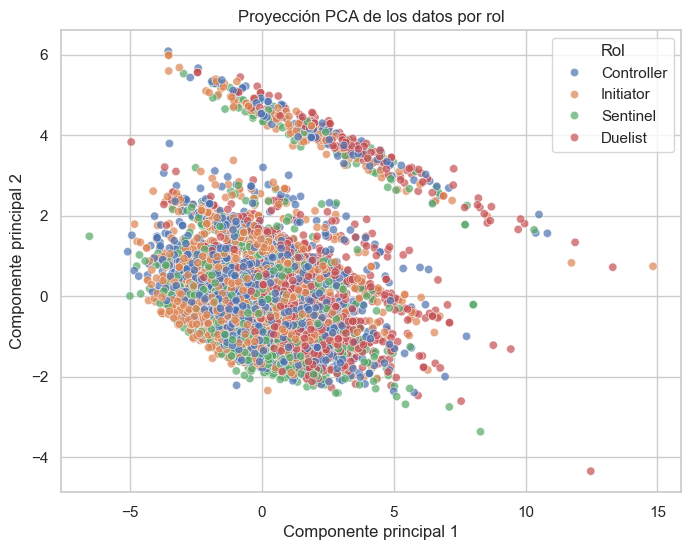
\includegraphics[width=0.8\textwidth]{data_charts/output9.png}
    \caption{Proyección PCA por rol}
    \label{fig:objetivos}
\end{figure}

\section{Generación de la variable objetivo}

Dado que el dataset original no contiene una etiqueta explícita de cumplimiento del rol, se adopta una estrategia de supervisión débil basada en reglas heurísticas. Para ello, primero se obtiene el rol del jugador mediante el mapeo del agente utilizado. Luego se define una función de scoring específica para cada rol.

Para el rol \textit{Duelist}, caracterizado por su impacto ofensivo y capacidad de apertura de rondas, el score se define como:

\[
Score_{Duelist} = 0.4 \cdot FKPR + 0.3 \cdot KPR - 0.2 \cdot FDPR + 0.1 \cdot ADR
\]

Para el rol \textit{Controller}, centrado en el control del mapa y apoyo al equipo, el score se calcula como:

\[
Score_{Controller} = 0.35 \cdot APR + 0.25 \cdot ADR + 0.2 \cdot KPR - 0.2 \cdot FDPR
\]

Para el rol \textit{Sentinel}, orientado a la defensa, supervivencia y control de zonas, el score se define como:

\[
Score_{Sentinel} = 0.3 \cdot Clutch\_Success + 0.25 \cdot (1 - FDPR) + 0.25 \cdot Survival + 0.2 \cdot APR
\]

Finalmente, para el rol \textit{Initiator}, enfocado en generar oportunidades para el equipo, el score se calcula como:

\[
Score_{Initiator} = 0.35 \cdot APR + 0.3 \cdot KPR + 0.2 \cdot ADR + 0.15 \cdot FKPR
\]

Una vez calculado el score bruto, este se normaliza al rango $[0,1]$ mediante \textit{MinMaxScaler}. El valor resultante se interpreta como la probabilidad de cumplimiento del rol y se utiliza como variable objetivo del modelo supervisado.

% FIGURA 2.10
\begin{figure}[H]
    \centering
    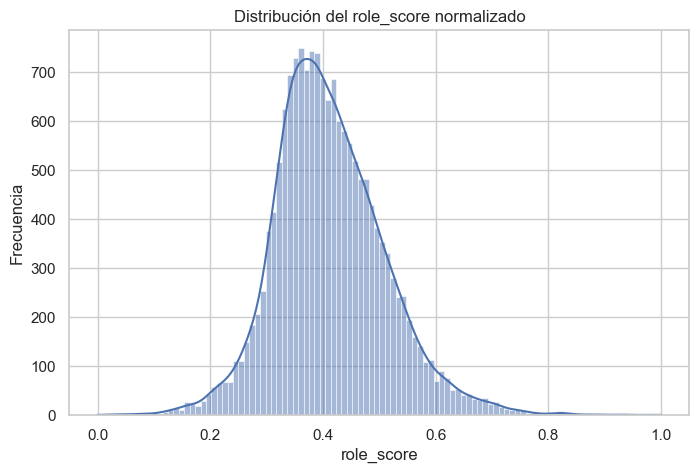
\includegraphics[width=0.8\textwidth]{data_charts/output10.png}
    \caption{Distribución del score normalizado}
    \label{fig:objetivos}
\end{figure}

\section{Modelo propuesto}

El problema se aborda como una tarea de regresión supervisada, ya que la variable objetivo \textit{role\_score} corresponde a un valor continuo normalizado en el intervalo $[0,1]$. Este valor representa la probabilidad estimada de cumplimiento del rol del jugador.

Con el objetivo de comparar distintos enfoques de modelado, se seleccionan tres algoritmos pertenecientes a familias diferentes:

\begin{itemize}
    \item \textbf{Linear Regression:} se utiliza como modelo base debido a su simplicidad e interpretabilidad. Permite establecer una referencia inicial para comparar el rendimiento de modelos más complejos.
    
    \item \textbf{KNN Regressor:} se incorpora como modelo basado en distancia. Su objetivo es estimar el cumplimiento del rol a partir de jugadores con características similares dentro del espacio de variables.
    
    \item \textbf{XGBoost Regressor:} se selecciona como modelo principal debido a su capacidad para trabajar con datos tabulares, capturar relaciones no lineales, manejar interacciones entre variables y ofrecer mecanismos de interpretación mediante importancia de características.
\end{itemize}

La inclusión de estos tres modelos permite comparar un enfoque lineal, un enfoque basado en similitud y un enfoque de ensamblaje basado en árboles. De esta manera, la selección final del modelo no se realiza de forma arbitraria, sino a partir de evidencia experimental obtenida mediante métricas de evaluación.

\subsection{Justificación de los modelos seleccionados}

La regresión lineal se utiliza como punto de partida porque permite evaluar si existe una relación aproximadamente lineal entre las variables del jugador y el \textit{role\_score}. Aunque es un modelo limitado para capturar interacciones complejas, resulta útil como línea base.

El modelo KNN Regressor permite analizar si jugadores con perfiles estadísticos similares presentan niveles similares de cumplimiento del rol. Este modelo es relevante en el contexto del sistema porque la comparación entre jugadores es una de las salidas esperadas de VRCE. Sin embargo, su rendimiento puede verse afectado por la escala de las variables, por lo que requiere normalización previa.

XGBoost Regressor se plantea como el modelo principal debido a que los datos presentan relaciones no lineales, variables con distinta escala, posibles outliers y dependencias entre métricas. Además, permite analizar la importancia relativa de las variables, lo cual resulta relevante para interpretar qué factores influyen en la estimación del cumplimiento del rol.

\subsection{Métricas de evaluación}

Dado que el objetivo del sistema es predecir un valor continuo en el intervalo $[0,1]$, se utilizan métricas propias de problemas de regresión. Las métricas seleccionadas son RMSE, MAE y $R^2$.

\begin{itemize}
    \item \textbf{RMSE (Root Mean Squared Error):} mide el error cuadrático medio entre el valor real y el valor predicho. Penaliza con mayor fuerza los errores grandes, por lo que resulta útil para detectar desviaciones importantes en la estimación del cumplimiento del rol.
    
    \[
    RMSE = \sqrt{\frac{1}{n}\sum_{i=1}^{n}(y_i - \hat{y}_i)^2}
    \]
    
    \item \textbf{MAE (Mean Absolute Error):} mide el error absoluto promedio. Su interpretación es directa, ya que indica cuánto se equivoca el modelo, en promedio, dentro de la escala normalizada del \textit{role\_score}.modelo.

    \[
    MAE = \frac{1}{n}\sum_{i=1}^{n}|y_i - \hat{y}_i|
    \]
    
    \item \textbf{R\textsuperscript{2} (Coeficiente de determinación):} mide la proporción de varianza explicada por el modelo. Un valor cercano a 1 indica que el modelo explica adecuadamente la variabilidad de la variable objetivo.

    \[
    R^2 = 1 - \frac{\sum_{i=1}^{n}(y_i - \hat{y}_i)^2}{\sum_{i=1}^{n}(y_i - \bar{y})^2}
    \]
    
\end{itemize}

Estas métricas permiten comparar los modelos desde tres perspectivas: magnitud del error, error promedio interpretable y capacidad explicativa general.

\section{Pipeline de preparación del dataset}

El flujo seguido durante el Hito 2 se resume en los siguientes pasos:

\begin{enumerate}
    \item Carga e inspección inicial del dataset.
    \item Análisis de tipos de datos, valores nulos y duplicados.
    \item Corrección de tipos y transformación de columnas porcentuales.
    \item Extracción de variables desde columnas compuestas.
    \item Mapeo de agentes a roles.
    \item Análisis exploratorio mediante estadísticas y visualizaciones.
    \item Identificación de sesgos y limitaciones del dataset.
    \item Ingeniería de variables.
    \item Generación del \textit{role\_score}.
    \item Normalización de la variable objetivo.
    \item Encoding de variables categóricas.
    \item Selección automática de características.
    \item Análisis PCA como técnica exploratoria.
    \item Entrenamiento del modelo supervisado
    \item Generación del output (probabilidad de cumplimiento y reporte)
\end{enumerate}

Este proceso permite transformar un dataset original no etiquetado en un conjunto de datos preparado para modelar la probabilidad de cumplimiento del rol.

\section{Repositorio del proyecto}

El desarrollo del sistema, incluyendo el procesamiento de datos, la generación de variables y el entrenamiento de modelos, se encuentra implementado en un repositorio de control de versiones. Este repositorio incluye notebooks de análisis exploratorio, scripts de preprocesamiento y entrenamiento, así como la definición completa del pipeline del sistema.

\begin{center}
\url{https://github.com/Nicocm30/DISIAG4_Proyecto-.git}
\end{center}

% -----------------------------------------------------------------
% HITO 3: ENTRENAMIENTO, VALIDACIÓN Y EVALUACIÓN DE MODELOS
% -----------------------------------------------------------------
\chapter{Entrenamiento, validación y evaluación de modelos}

En este capítulo se presenta el proceso de entrenamiento, validación y comparación de los modelos de aprendizaje automático utilizados en el sistema \textit{VRCE -- Valorant Role Compliance Evaluation}. Asimismo, se describen las métricas de evaluación empleadas, la optimización de hiperparámetros, el análisis de errores y la interpretación de los resultados desde la perspectiva del dominio competitivo de \textit{Valorant}.

\section{Preparación de datos para el modelado}

Una vez finalizada la fase de limpieza, análisis exploratorio y selección de características, se construye el conjunto final de variables utilizado durante el entrenamiento de los modelos.

Con el objetivo de reducir redundancias y conservar únicamente variables relevantes para la predicción del \textit{role\_score}, se emplea \textit{SelectKBest} utilizando la función estadística \textit{f\_regression}. Este proceso permite seleccionar automáticamente las variables con mayor relación estadística respecto a la variable objetivo.

Las variables seleccionadas incluyen métricas ofensivas, métricas de soporte, métricas de riesgo, métricas críticas y variables contextuales relacionadas con el agente y el rol.

Posteriormente, el dataset se divide en dos subconjuntos:

\begin{itemize}
    \item \textbf{Conjunto de entrenamiento:} utilizado para entrenar y optimizar los modelos.
    \item \textbf{Conjunto de prueba:} utilizado para evaluar la capacidad de generalización de los modelos sobre datos no vistos.
\end{itemize}

La división se realiza utilizando una proporción del 80\% para entrenamiento y 20\% para prueba, empleando una semilla fija para garantizar reproducibilidad experimental.

\section{Modelos evaluados}

Con el objetivo de comparar diferentes enfoques de aprendizaje automático, se seleccionan tres modelos pertenecientes a familias distintas:

\begin{itemize}
    \item \textbf{Linear Regression}
    \item \textbf{KNN Regressor}
    \item \textbf{XGBoost Regressor}
\end{itemize}

La inclusión de múltiples familias de modelos permite comparar enfoques lineales, modelos basados en distancia y modelos basados en ensamblaje de árboles.

\subsection{Linear Regression}

La regresión lineal se utiliza como modelo base debido a su simplicidad e interpretabilidad. Este modelo asume relaciones lineales entre las variables predictoras y la variable objetivo.

Aunque sus capacidades para capturar relaciones complejas son limitadas, resulta útil como referencia inicial para determinar si modelos más avanzados ofrecen mejoras significativas.

\subsection{KNN Regressor}

El modelo \textit{K-Nearest Neighbors Regressor} se utiliza para analizar el comportamiento del sistema bajo un enfoque basado en similitud. Este algoritmo estima el valor de salida a partir de jugadores con características estadísticas cercanas dentro del espacio de variables.

El uso de KNN resulta relevante porque el problema de cumplimiento del rol involucra comparaciones implícitas entre jugadores con perfiles similares. Sin embargo, el rendimiento del modelo depende fuertemente de la escala de las variables y puede verse afectado por la dimensionalidad del dataset.

\subsection{XGBoost Regressor}

XGBoost Regressor se selecciona como modelo principal debido a su capacidad para trabajar con datos tabulares, modelar relaciones no lineales y manejar interacciones complejas entre variables.

Además, XGBoost presenta varias ventajas relevantes para este problema:

\begin{itemize}
    \item Robustez frente a outliers.
    \item Buen rendimiento sobre datasets tabulares.
    \item Capacidad de capturar relaciones no lineales.
    \item Posibilidad de interpretar importancia de variables.
    \item Capacidad de generalización en presencia de variables heterogéneas.
\end{itemize}

Estas características resultan especialmente importantes debido a que el comportamiento de los jugadores depende de múltiples factores tácticos y estadísticos que no necesariamente presentan relaciones lineales.

\section{Entrenamiento y evaluación inicial}

Cada modelo es entrenado utilizando el conjunto de entrenamiento y posteriormente evaluado sobre el conjunto de prueba.

La Tabla \ref{tab:model_comparison} presenta la comparación inicial de modelos utilizando RMSE, MAE y $R^2$.

% TABLA RESULTADOS
\begin{table}[H]
    \centering
    \caption{Comparación inicial de modelos}
    \label{tab:model_comparison}
    \begin{tabular}{|l|c|c|c|}
        \hline
        \textbf{Modelo} & \textbf{RMSE} & \textbf{MAE} & \textbf{$R^2$} \\ \hline
        Linear Regression & 0.044868 & 0.031268 & 0.741759 \\ \hline
        KNN Regressor & 0.074165 & 0.057280 & 0.294425 \\ \hline
        XGBoost Regressor & 0.015952 & 0.009656 & 0.967357 \\ \hline
    \end{tabular}
\end{table}

Los resultados iniciales muestran diferencias significativas entre modelos. Los enfoques lineales presentan limitaciones para capturar relaciones complejas entre variables, mientras que modelos más flexibles como XGBoost logran representar mejor la variabilidad del dataset.

% FIGURA COMPARACIÓN MODELOS
\begin{figure}[H]
    \centering
    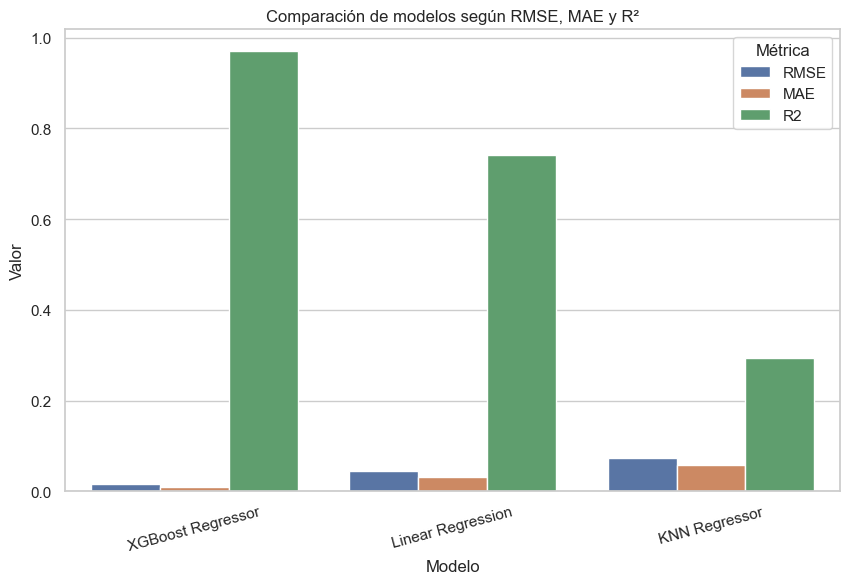
\includegraphics[width=0.75\textwidth]{models_charts/comparacion_modelos.png}
    \caption{Comparación de modelos mediante métricas RMSE, MAE y $R^2$.}
    \label{fig:model_comparison}
\end{figure}

\section{Optimización de hiperparámetros}

La optimización de hiperparámetros se realiza con el objetivo de mejorar la capacidad de generalización de los modelos y reducir errores de predicción sobre datos no vistos. Aunque los algoritmos seleccionados poseen configuraciones por defecto funcionales, su rendimiento puede variar significativamente dependiendo de la naturaleza del dataset, la distribución de las variables y la complejidad de las relaciones presentes en los datos.

En el contexto del sistema VRCE, las variables utilizadas presentan relaciones no lineales, distribuciones heterogéneas, presencia de outliers y diferencias de escala entre métricas ofensivas, defensivas y contextuales. Debido a ello, resulta necesario ajustar los hiperparámetros de los modelos para controlar aspectos como complejidad, sensibilidad al ruido, capacidad de aprendizaje y riesgo de sobreajuste.

Para este proceso se utiliza \textit{GridSearchCV}, una técnica de búsqueda exhaustiva que evalúa múltiples combinaciones de hiperparámetros mediante validación cruzada. La selección de este método se justifica porque permite:

\begin{itemize}
    \item Explorar sistemáticamente diferentes configuraciones del modelo.
    \item Comparar configuraciones utilizando una misma métrica de evaluación.
    \item Reducir el riesgo de seleccionar hiperparámetros de forma arbitraria.
    \item Mejorar la reproducibilidad experimental.
    \item Disminuir el riesgo de sobreajuste sobre el conjunto de entrenamiento.
\end{itemize}

La validación cruzada utilizada por \textit{GridSearchCV} permite evaluar cada combinación sobre diferentes particiones del dataset, obteniendo una estimación más estable del rendimiento esperado del modelo.

\subsection{Optimización de KNN Regressor}

En el caso de KNN Regressor, se optimizan los hiperparámetros \textit{n\_neighbors} y \textit{weights}, ya que ambos controlan directamente el comportamiento del modelo durante la estimación de vecinos similares.

\begin{itemize}
    \item \textbf{n\_neighbors:} determina la cantidad de vecinos utilizados para realizar la predicción.
    
    Valores pequeños permiten capturar patrones locales con mayor sensibilidad, pero pueden incrementar la variabilidad y el riesgo de sobreajuste. Por el contrario, valores más altos generan predicciones más estables, aunque pueden suavizar excesivamente diferencias importantes entre jugadores.
    
    En este proyecto se evalúan los valores 3, 5, 7 y 9, ya que representan configuraciones suficientemente pequeñas para conservar sensibilidad local sin introducir una complejidad computacional excesiva.
    
    \item \textbf{weights:} define cómo contribuyen los vecinos a la predicción final.
    
    La opción \textit{uniform} asigna el mismo peso a todos los vecinos, mientras que \textit{distance} otorga mayor importancia a los vecinos más cercanos. Esta comparación resulta relevante debido a que algunos jugadores pueden presentar perfiles estadísticos muy similares dentro de un mismo rol.
\end{itemize}

\subsection{Optimización de XGBoost Regressor}

Para XGBoost Regressor se seleccionan hiperparámetros relacionados con capacidad de aprendizaje, complejidad estructural y velocidad de convergencia del modelo.

\begin{itemize}
    \item \textbf{n\_estimators:} controla la cantidad de árboles utilizados en el ensamblaje.
    
    Un número mayor de árboles puede mejorar la capacidad predictiva, pero también incrementa el riesgo de sobreajuste y el costo computacional. Por esta razón se evalúan configuraciones moderadas de 100 y 200 árboles.
    
    \item \textbf{max\_depth:} determina la profundidad máxima de cada árbol.
    
    Profundidades pequeñas limitan la complejidad del modelo y favorecen la generalización, mientras que profundidades muy altas pueden generar árboles excesivamente específicos del conjunto de entrenamiento.
    
    En este proyecto se evalúan profundidades de 3, 5 y 7, ya que permiten explorar distintos niveles de complejidad manteniendo un equilibrio razonable entre capacidad de representación y riesgo de sobreajuste.
    
    \item \textbf{learning\_rate:} controla la magnitud de las actualizaciones realizadas durante el proceso de boosting.
    
    Tasas de aprendizaje bajas producen modelos más estables y con mejor capacidad de generalización, aunque requieren más iteraciones. En cambio, tasas demasiado altas pueden provocar convergencia inestable.
    
    Por esta razón se seleccionan los valores 0.01, 0.05 y 0.1, los cuales representan configuraciones comúnmente utilizadas en problemas de regresión sobre datos tabulares.
\end{itemize}

La combinación de estos hiperparámetros permite explorar distintos niveles de complejidad y capacidad de aprendizaje, manteniendo un equilibrio entre rendimiento predictivo, estabilidad y generalización.

\section{Evaluación del modelo final}

Tras el proceso de optimización, el modelo final seleccionado corresponde a XGBoost Regressor, debido a que presenta el mejor equilibrio entre error y capacidad explicativa.

La Tabla \ref{tab:final_metrics} muestra las métricas obtenidas por el modelo final.

% TABLA MODELO FINAL
\begin{table}[H]
    \centering
    \caption{Resultados del modelo final XGBoost}
    \label{tab:final_metrics}
    \begin{tabular}{|l|c|}
        \hline
        \textbf{Métrica} & \textbf{Valor} \\ \hline
        RMSE & 0.0127 \\ \hline
        MAE & 0.0080 \\ \hline
        $R^2$ & 0.9792 \\ \hline
    \end{tabular}
\end{table}

\section{Análisis visual del rendimiento}

Con el objetivo de evaluar visualmente el comportamiento de los modelos, se generan gráficos de predicción real vs predicción estimada y análisis de residuos.

\subsection{Real vs Predicted}

Los gráficos de valores reales vs predichos permiten analizar la capacidad del modelo para aproximar correctamente el \textit{role\_score}. Un modelo ideal presentaría los puntos alineados sobre la diagonal principal.

% FIGURA REAL VS PREDICTED
\begin{figure}[H]
    \centering
    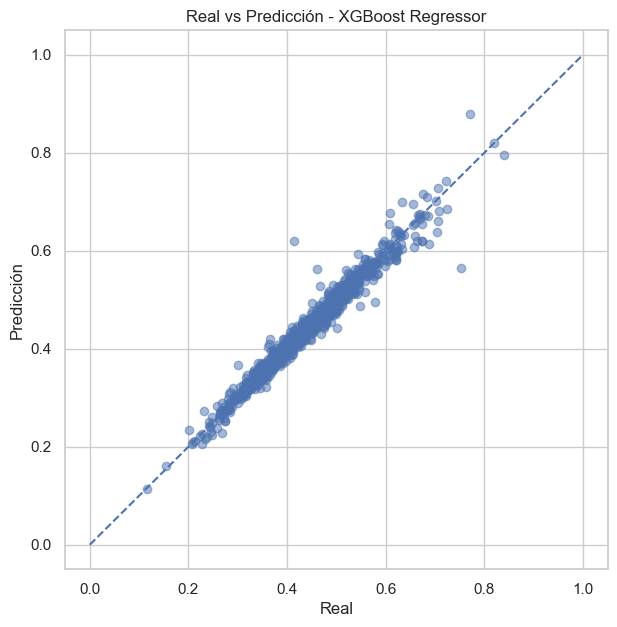
\includegraphics[width=0.7\textwidth]{models_charts/real_vs_predicted_xgb.png}
    \caption{Comparación entre valores reales y predichos para XGBoost Regressor.}
    \label{fig:real_vs_predicted}
\end{figure}

\subsection{Análisis de residuos}

El análisis de residuos permite estudiar la distribución de errores generados por el modelo. Una distribución centrada alrededor de cero sugiere que el modelo no presenta sesgos sistemáticos significativos.

% FIGURA RESIDUOS
\begin{figure}[H]
    \centering
    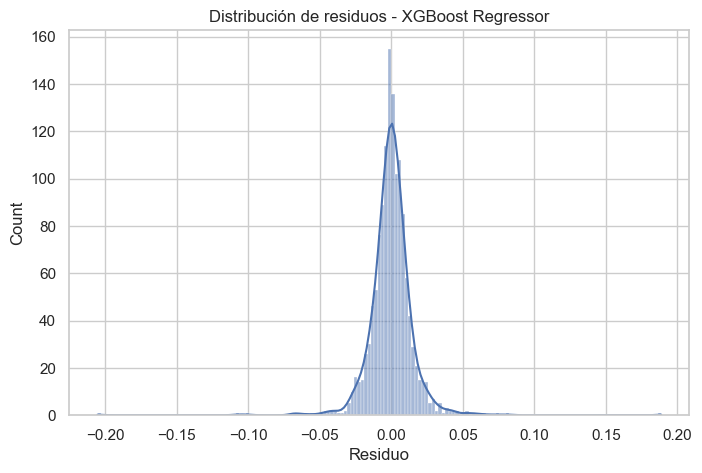
\includegraphics[width=0.7\textwidth]{models_charts/residuals_xgb.png}
    \caption{Distribución de residuos del modelo XGBoost Regressor.}
    \label{fig:residuals}
\end{figure}

\section{Importancia de variables}

Una de las ventajas principales de XGBoost es la posibilidad de analizar la importancia relativa de las variables utilizadas durante el entrenamiento.

El análisis de importancia muestra qué métricas tienen mayor influencia sobre la estimación del cumplimiento del rol. Variables ofensivas como \textit{Kills Per Round} y \textit{Average Damage Per Round} presentan alta relevancia para roles agresivos, mientras que variables relacionadas con clutch y supervivencia adquieren mayor importancia en roles defensivos.

% FIGURA FEATURE IMPORTANCE
\begin{figure}[H]
    \centering
    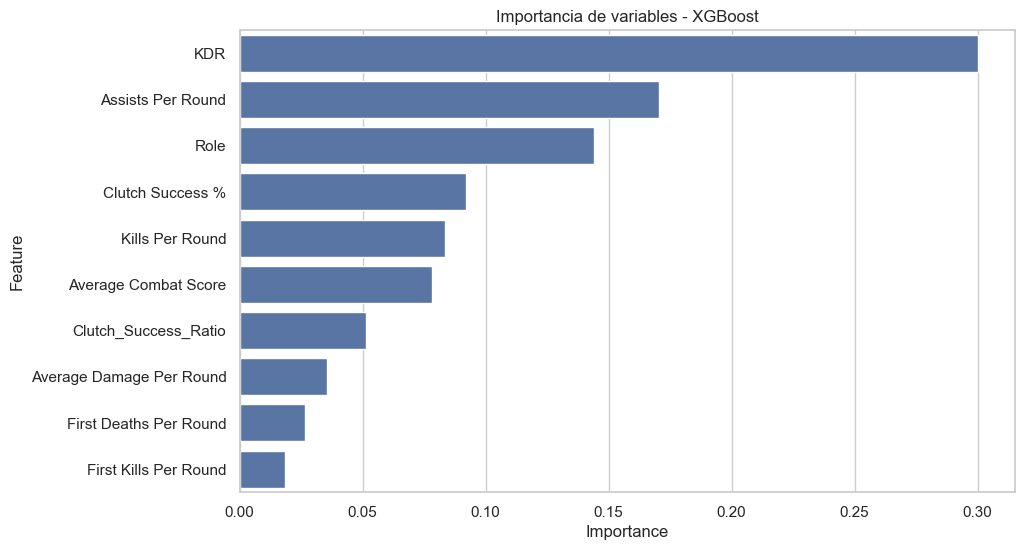
\includegraphics[width=0.8\textwidth]{models_charts/feature_importance_xgb.png}
    \caption{Importancia de variables en el modelo XGBoost Regressor.}
    \label{fig:feature_importance}
\end{figure}

\section{Impacto sobre métricas del dominio}

Los resultados obtenidos muestran que el modelo logra capturar comportamientos coherentes con el dominio competitivo de \textit{Valorant}.

En roles como \textit{Duelist}, las variables ofensivas y de apertura de rondas tienen mayor impacto en la estimación del cumplimiento del rol. En cambio, para roles como \textit{Sentinel}, variables relacionadas con supervivencia y clutch adquieren mayor relevancia.

Esto indica que el modelo no se limita a aprender correlaciones superficiales, sino que logra aproximar parcialmente responsabilidades tácticas asociadas a cada rol.

Además, el uso de variables contextuales como agente y rol permite reducir comparaciones incorrectas entre jugadores con funciones distintas dentro del equipo.

\section{Análisis de errores}

Con el objetivo de comprender las limitaciones del modelo y detectar escenarios donde las predicciones presentan menor precisión, se realiza un análisis específico sobre los errores generados por el modelo final XGBoost Regressor.

Para ello, se calcula el error absoluto entre el valor real del \textit{role\_score} y el valor predicho:

\[
Absolute\ Error = |y - \hat{y}|
\]

El análisis de la distribución de errores permite observar que la mayoría de las predicciones presentan desviaciones relativamente bajas, mientras que un conjunto reducido de registros concentra los errores más altos.

% FIGURA ERROR DISTRIBUTION
\begin{figure}[H]
    \centering
    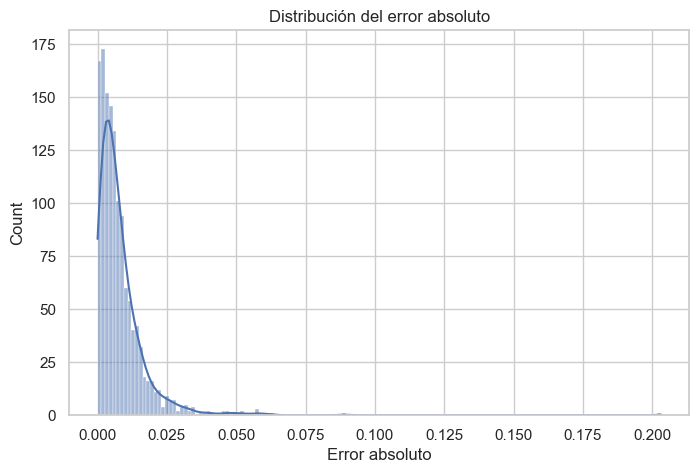
\includegraphics[width=0.7\textwidth]{models_charts/absolute_error_distribution.png}
    \caption{Distribución del error absoluto del modelo XGBoost Regressor.}
    \label{fig:absolute_error_distribution}
\end{figure}

Los errores más elevados aparecen principalmente en jugadores cuyos comportamientos estadísticos no se ajustan completamente al patrón esperado de su rol. Esto incluye escenarios como:

\begin{itemize}
    \item Jugadores con estilos híbridos entre roles.
    \item Desempeños extremadamente agresivos o conservadores.
    \item Métricas ofensivas inconsistentes respecto al rol asignado.
    \item Partidas atípicas con alto impacto individual.
\end{itemize}

Por ejemplo, algunos registros presentan diferencias significativas entre el valor real y el valor estimado del \textit{role\_score}, lo que sugiere que ciertos comportamientos competitivos no pueden ser explicados completamente mediante las métricas disponibles.

Adicionalmente, se analiza el error promedio por rol para identificar posibles diferencias en la capacidad predictiva del modelo según la función táctica del jugador.

% FIGURA ERROR POR ROL
\begin{figure}[H]
    \centering
    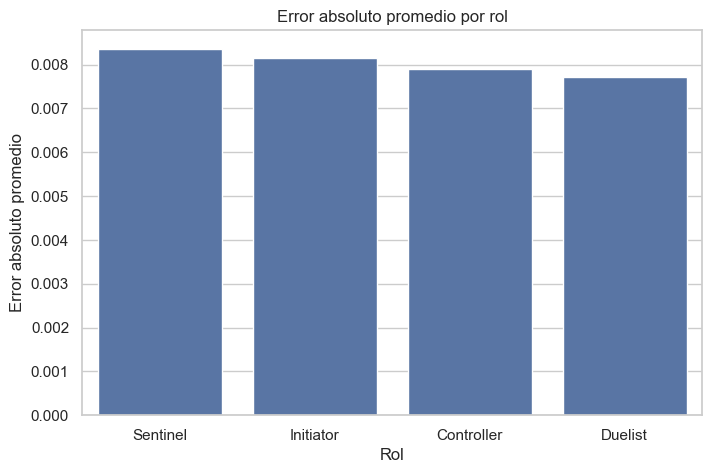
\includegraphics[width=0.7\textwidth]{models_charts/error_by_role.png}
    \caption{Error absoluto promedio por rol.}
    \label{fig:error_by_role}
\end{figure}

Este análisis muestra que algunos roles presentan mayor dificultad de modelado debido a la naturaleza de sus responsabilidades dentro del juego. Roles como \textit{Controller} o \textit{Initiator} pueden involucrar contribuciones tácticas difíciles de representar únicamente mediante estadísticas tradicionales.

Asimismo, el análisis entre predicción y error absoluto permite observar que el modelo tiende a presentar mayor incertidumbre en jugadores con valores extremos de cumplimiento del rol.

% FIGURA ERROR VS PREDICTION
\begin{figure}[H]
    \centering
    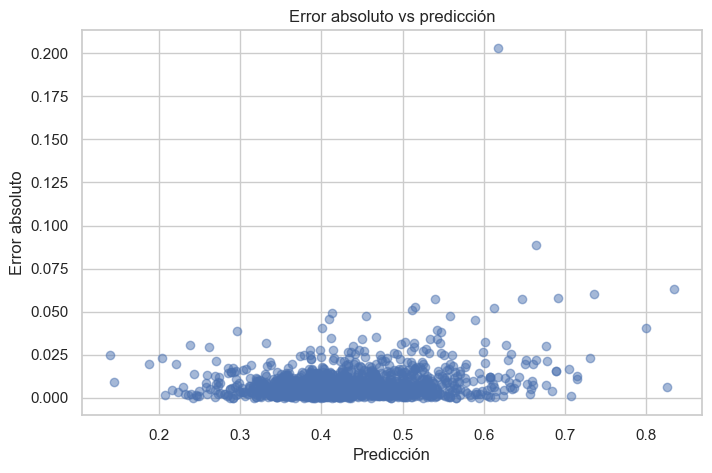
\includegraphics[width=0.7\textwidth]{models_charts/error_vs_prediction.png}
    \caption{Relación entre predicción y error absoluto.}
    \label{fig:error_vs_prediction}
\end{figure}

Estas limitaciones están directamente relacionadas con las restricciones del dataset. El sistema no dispone de información espacial, uso detallado de habilidades, comunicación del equipo ni análisis táctico derivado de video. Como consecuencia, algunos aspectos fundamentales del cumplimiento del rol no pueden ser capturados completamente por el modelo.

A pesar de ello, el comportamiento general de los errores sugiere que el modelo logra aproximar de forma razonable patrones funcionales asociados al desempeño competitivo de los jugadores.

% =================================================================
% BIBLIOGRAFÍA (Añadir fuentes bibliográficas)
% =================================================================
\newpage
\begin{thebibliography}{99}

    \bibitem{riot_api}
    Riot Games. (2024). 
    \textit{Riot Games Developer Portal}. Recuperado de https://developer.riotgames.com/
    
    \bibitem{henrik_api}
    HenrikDev. (2024). 
    \textit{Valorant API Documentation}. Recuperado de https://docs.henrikdev.xyz/
    
    \bibitem{tracker}
    Tracker Network. (2024). 
    \textit{Valorant Tracker}. Recuperado de https://tracker.gg/valorant
    
    \bibitem{vlr}
    VLR.gg. (2024). 
    \textit{Valorant Esports Statistics}. Recuperado de https://www.vlr.gg/
    
    \bibitem{james}
    James, G., Witten, D., Hastie, T., \& Tibshirani, R. (2021). 
    \textit{An Introduction to Statistical Learning} (2nd ed.). Springer.
    
    \bibitem{geron}
    Géron, A. (2022). 
    \textit{Hands-On Machine Learning with Scikit-Learn, Keras, and TensorFlow} (3rd ed.). O'Reilly Media.
    
    \bibitem{bishop}
    Bishop, C. M. (2006). 
    \textit{Pattern Recognition and Machine Learning}. Springer.
    
    \bibitem{breiman}
    Breiman, L. (2001). Random forests. 
    \textit{Machine Learning}, 45(1), 5–32.
    
    \bibitem{xgboost}
    Chen, T., \& Guestrin, C. (2016). XGBoost: A scalable tree boosting system. 
    \textit{Proceedings of the 22nd ACM SIGKDD International Conference on Knowledge Discovery and Data Mining}.
    
    \bibitem{feature_engineering}
    Kuhn, M., \& Johnson, K. (2019). 
    \textit{Feature Engineering and Selection}. Chapman and Hall/CRC.
    
    \bibitem{sports_analytics}
    Gudmundsson, J., \& Horton, M. (2017). Spatio-temporal analysis of team sports. 
    \textit{ACM Computing Surveys}, 50(2).
    
    \bibitem{esports}
    Block, F., et al. (2018). Esports analytics: A framework for player performance evaluation. IEEE Conference.

\end{thebibliography}

\end{document}
